\documentclass[letterpaper] {article}
\usepackage{stylesheet}
\usepackage{verbatim}
\usepackage{xcolor}

\begin{document}

	\lhead{CPSC 210 Summary Notes}
	\title{CPSC 210 Summary Notes}
	\author{Markus de Medeiros}
	\maketitle

    \begin{abstract}
        This is a summary of the basic content of CPSC 210. All credit is owed to the instructors of the 2019WT2 session of CPSC 210 at the University of British Columbia, or the respective owners. This document does not cover the practical skills of this class (such as debugging or working in intellij) and should not be taken as wholeheartedly comprehensive. 
    \end{abstract}

    \begin{comment}
    
    \section{Section}

    \subsection{Lesson}
    \begin{framed}
        \begin{center}
            Design Principle: Principle
        \end{center}
        Information
    \end{framed}

    \begin{lstlisting}
        public static void main(String args[]) {
            // Java Code
        }
    \end{lstlisting}

    \end{comment}

    \section{Basics}

    \subsection{Program Structure}
    \begin{itemize}
        \item Basic Java files are called \textbf{classes}.
        \item Folders, in Java, are called \textbf{packages}.
        \item The runnable class has a \textbf{main} method.
        \item Classes see other classes with \textbf{import statements}. 
    \end{itemize}

    We can represent this diagramatically, but we will probably use UML diagrams instead. \\

    \subsection{Methods, Calls, Call Graphs}
    
    \begin{itemize}
        \item A \textbf{call graph} shows us how a method is run step by step: 
            \begin{center}
                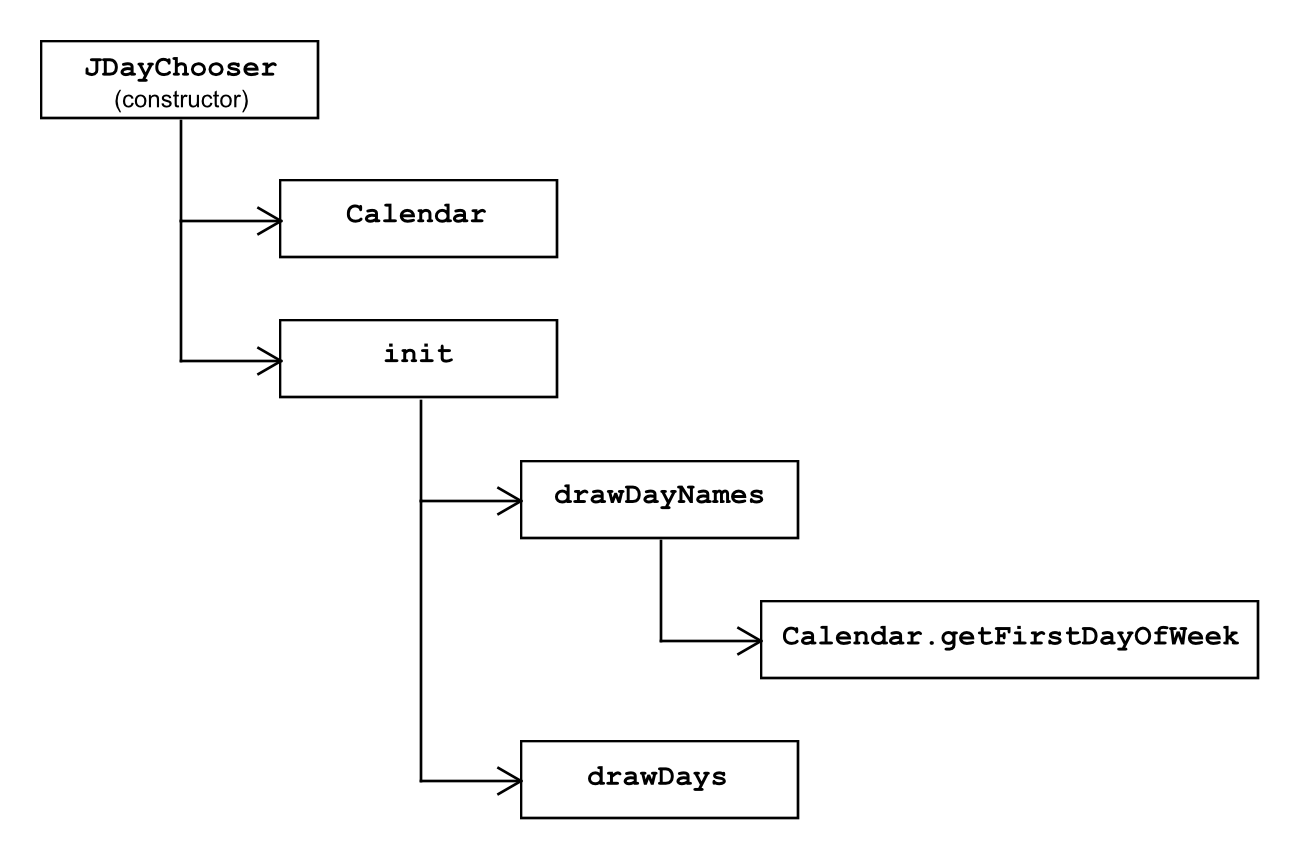
\includegraphics[width=3in]{callgraph}
            \end{center}
            Each method in a call graph must appear only once (recursion becomes loops).
    \end{itemize}

    \subsection{Classes, Objects, and Variables}
    
    \begin{framed}
        \begin{center}
            Design Principle: Object Orientation
        \end{center}
        Java is built around \textbf{classes} which encode the data and behavior of a single concept. Creating an \textbf{instance} of a class gives the instance it's own copy of all of the classes data and methods.
    \end{framed}

    \begin{itemize}
        \item A \textbf{variable} is a symbol, with a \textbf{type}, which has a holder for an object of that type. 
        \item We \text{assign} a value to a type to out the value into it's holder. 
        \item Primitive types (int, bool, \dots) exist in the holder. Objects are different, a variable is given a reference to an object (not the object itself). 
        \item If a non primitive variable $a$ is assigned to another non primitive variable $b$, then $a$ is defined to be a reference to whatever $b$ refers to at the time of instantiation. If $b$ changes to point to a different object, $a$ will not update to point to that new object (arrows do not chain, they copy).
        \item An object is \textbf{active} if it has been instantiated. 
        \item Within a class, global variables are called \textbf{fields}. 
        \item The \textbf{static} keyword denotes a method to live outside of instances, and can be called without reference to any particular object. 
    \end{itemize}

    \subsection{Data Flow}
    \begin{itemize}
        \item Paramaters of methods are local variables. This means that a primitive paramater will copy and not mutate, but non primitive objects (which are copied as references) will indeed mutate.
        \item A similar principle applies to \textbf{return values}, which also return references to objects. 
        \item A constructor is a function in a class which returns a new object of that type. 
        \item The keyword \textbf{this} is used to refer to the instance of the object. It is like a variable in an object with a reference to itself. 
    \end{itemize}

    \subsection{Excecution of a Method}
    \begin{itemize}
        \item Methods excecute their lines of code sequentially, and can be changed by control structures.
        \item We use a \textbf{flowchart} to encode the sequence of operations a method preforms. A cheat sheet (taken from edX) is included in the root folder of this document. 
        \item In summary of flowcharts: \textbf{code block} is a rectangle, and \textbf{if} statement is a diamond (outgoing edges labelled T/F), a \textbf{switch} or \textbf{else if/else} block are linked diamonds, a \textbf{while} (or \textbf{do/while}) loop is a diamond linked to itself, a \textbf{for each} loop is a loop labelled \textit{collection hasNext()?} and a \textbf{for} loop is like a while loop with additional code before the loop check. 
    \end{itemize}
    
    \newpage    
    \section{Abstraction}

    \subsection{Specification and Using a Data Abstraction}
    
    \begin{framed}
        \begin{center}
            Design Principle: Abstraction 
        \end{center}
        \textbf{Abstraction} is the principle of intentionally hiding inessential details of something beihind an interface or container, so that the container can be treated exactly as the object it represents without concern for the details of it's implementation. \textbf{Statment abstraction} is applying labels to data or basic methods (like machiene code). \textbf{Functional abstraction} is applying a label to a function which may be implemented elsewhere. \textbf{Data abstraction} is applying a label to a piece of data which may include methods and fields. \\

        It is helpful for long term reusability and code sustainability to keep the public interface focused on the towards of the object itself. The public interface of an object should be designed to be stable over time. 
    \end{framed}

    \begin{itemize}
        \item The \textbf{visible interface} (public in Java) of an abstraction are the things that are designed to be interacted with, the \textbf{invisible implementation} (private in Java) are the things that are designed to be hidden. 
        \item It is good practice for essential fields (foe example width or height) to be private, and to create \textbf{getter} and \textbf{setter} interfaces to change them instead.
    \end{itemize}

    \begin{framed}
        \begin{center}
            Design Principle: Designing an Abstraction
        \end{center}
        There are four steps to black box design: 
        \begin{enumerate}
            \item \textbf{Specify} what the abstraction provides.
            \item Consider the \textbf{use} of the data abstraction.
            \item \textbf{Test} the abstraction based on these uses (correct and incorrect).
            \item \textbf{Implement} the abstraction to pass the tests. 
        \end{enumerate}
    \end{framed}
    \begin{itemize}
        \item In the specification phase, we write three clauses for our methods. The \textbf{requires} clause outlines conditions for correct operation, the \textbf{modifies} clause outlines what data the method changes, and the \textbf{effects} clause outlines what the method is designed to do. 
        \item The modifies clause must keep in mind that non-primitive objects are passed by reference, so can have side effects on those objects. Additionally, \textbf{this} means that the object may mutate itself. 
        \item Empty clauses need not be written. 
    \end{itemize}

    \subsection{Testing a Data Abstraction}
    \begin{framed}
        \begin{center}
            Design Principle: Black Box Testing
        \end{center}
        Black box testing is designing tests strictly on the abstraction level. It serves as a way to encode the specification in code, and to ensure that the abstraction (public interface) is remaining functional as designed over long periods of development. 
    \end{framed}

    \begin{itemize}
        \item Good testing has \textbf{branch coverage} (no cases missed) and \textbf{boundary checking}.
    \end{itemize}

   \begin{framed}
        \begin{center}
            Design Principle: Testability
        \end{center}
        An abstraction is \textbf{testable} if it includes methods to determine if a the other methods operated succesfully. An abstraction with poor testability would have methods which require details of the internal implementation to be tested. 
    \end{framed}

    \subsection{Implementing a Data Abstraction}
    \begin{itemize}
        \item Implementatation of an abstraction is the process of writing the code (or stubs) for the interface, running tests, and fixing code for failing tests. If a test suite is comprehensive, any solution satisfying all tests is valid. 
        \item If all the fields are private, this process even allows for the types of fields to be modified and maintain a valid solution. This is helpful for \textbf{collections} in Java, which have different types for different purposes which may arise (more on collections below).
    \end{itemize}

    \subsection{Types and Interfaces}
    \begin{itemize}
        \item \textbf{Inheritance} is a way to encode similarities between types, and also to avoid code duplication. 
        \item \textbf{Interfaces} are special classes which can have a public interface but no implementation (so cannot be instantiated). \textbf{Abstract Classes} have a public interface and an an implementation but cannot be instantiated. 
        \item Both of these serve to abstract similarities between types through inheritance: for example if type $A$ and $B$ both have a method $c$, we can avoid duplication by having $A$ and $B$ \textbf{implement} an abstract class or interface $C$ which has details for $c$. 
        \item If a type $A$ is a special version of another type $B$ with additional or modified behavior, we would use the inheritance $A$ \textbf{extends} $B$. A child class can only extend one parent class, but a parent class can have many children. 
        \item In UML, a class is a named box with a list of important operations (in the public interface) and a tag \textit{abstract} or \textit{interface} if it applies. 
        \item In UML implements is represented by a dotted line with a hollow arrowhead at the supertype, and extends is represented by a solid line with a hollow arrowhead at the supertype. 
            \begin{center}
                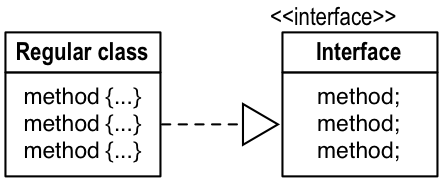
\includegraphics[width=1.5in]{implements} \\
                \medskip
                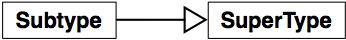
\includegraphics[width=1.5in]{extends}
        \end{center}
        \item Suptypes are always substitutable for a supertype. 
        \item Classes are instantiated with \textbf{apparent} and \textbf{actual} types. An object can be of any actual type which is a subtype of the apparent type, and must only use the functionality of the apparent type.  
            \begin{lstlisting}
                ApparentType name = new ActualType(paramaters)
            \end{lstlisting}
        \item Concrete types must have all abstract methods implemented. 
        \item Paramaters of methods check for the apparent type of an object (at compile time). Thus, methods can take several types (a concept called \textbf{subtype polymorphism}).
    \end{itemize}

    \subsection{Multiple Interfaces}
    \begin{itemize}
        \item A class can extend multiple interfaces. If two interfaces have methods with the same name (and paramaters) there can only be one implementation for both. This is a potential design issue, if two methods with the same name in different interfaces have different intended behaviors.
        \item In some implementations the apparent type of an object can be \textbf{casted} to the actual type if substitution is violated, but in general this is a symptom of poor type hierarchy design.
    \end{itemize}

    \subsection{Extends and Overriding}
    \begin{itemize}
        \item Extended subclasses inherit public and protected fields and methods of their parent classes.
        \item \textbf{Method Dispatch} is the process of searching for an implementation for a mehthod. If the actual type of an object does not have an implementation, Java seaches up the type hierarchy for an implementation.  
        \item A subclass can implement a supertype method and it will \textbf{override} the implementation during method dispatch. 
        \item In a subclass the \textbf{super} keyboard accesses supertype methods. This is particularly helpful for subclasses which augment superclass behavior, using methods of the same name. 
    \end{itemize}

    \subsection{Abstract classes and Overloading Methods}
    \begin{itemize}
        \item The \textbf{abstract} keyword before methods in abstract classes allow a method with no default implementation but that must be implemented in concrete subclasses. 
        \item A method is \textbf{overloaded} if there are two methods with the same name but different paramater lists in scope. Java will view these as seperate methods, but it is often helpful to have overloaded methods for allow some flexibility in paramater types. 
        \item Abstract classes must be tested with abstract or overridden test classes. 
        \item Fields should not be redeclared in subclasses. 
    \end{itemize}


    \newpage
    \section{Construction} 

    \subsection{Throwing and Catching Exceptions}
    \begin{framed}
        \begin{center}
            Design Principle: Robust Code
        \end{center}
        Code is \textbf{robust} if it preforms well over a large domain of inputs. In Java, Robust code will have small \textit{requires} clauses, and will be able to handle unexpected errors that occur even when the \textit{requires} clause is met. 
    \end{framed}

    \begin{itemize}
        \item In Java, \textbf{exceptions} are objects which represent unhandled conditions in code. 
        \item When a functions \textbf{throws} an exception, it passes it the exception up the call stack. 
        \item We can write new exceptions by extending Exception classes 
            \begin{center}
                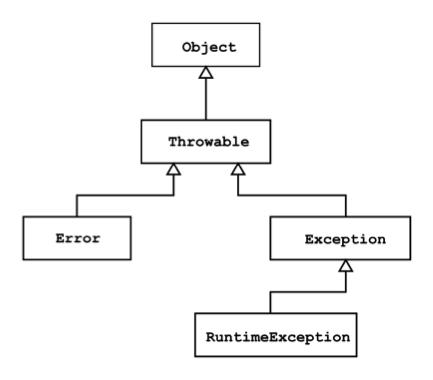
\includegraphics[width=3in]{exceptions}
            \end{center}
            and throw a new exception with
            \begin{lstlisting}
                throw new ExceptionType(paramaters)
            \end{lstlisting}
            It can be helpful to override the constructor with a string describing the error. 
        \item Exceptions that may throw an exception of type $E$ without catching it are denoted with the \textbf{throws} $E$ keyword in the method signature. 
        \item Exceptions can be caught with \textbf{try/catch} blocks. Every \textbf{catch} block catches exception by exception type.. A \textbf{finally} clause can be used to run code regardless of if an exception is thrown, but before the exception is passed up the stack trace. 
        \item It is possible, and sometimes helpful, for catch blocks to throw new exceptions themselves. However each try/catch block will only catch one exception, even if that exception throws a new exception which is catchable below in the block. 
        \item If main throws or does not catch an exception, the program will crash. 
    \end{itemize}

    \subsection{Exception Hierarchy/Unchecked Exceptions/Assertions}
    \begin{itemize}
        \item Duplicate catch blocks can be abstracted away by having exceptions extend other exceptions. By substitution, Java catch blocks will also catch all subtypes of exceptions. It also follows that the order of catch blocks is important. 
        \item \textbf{Runtime (Unchecked) Exceptions} do not need to be caught. An unchecked exception can be caught with a try/catch block, and if an unchecked exception is thrown in a try/catch/finally block the finally clause will be run and the exception will be passed up the call stack. 
        \item Runtime exceptions are used for errors that rarely, but sometimes do, happen. 
        \item A \textbf{class invariant} is a statement (written at the top of the class) which must be maintained by all functions. 
        \item To ensure class invariants are maintained, we use \textbf{assert} statements to check class invariants at points in our code, and these statements can be turned off by the compiler so they do not slow down the final program. 
    \end{itemize}
    
    \subsection{Testing Exceptions}
    \begin{itemize}
        \item To test if exceptions are thrown, we use try/catch blocks in our test classes. If exceptions should be thrown but aren't, or if an exception is thrown but isn't, the \textbf{fail(message)} method can be used to indicate an incorrectly exception. 
    \end{itemize}

    \subsection{Extracting Hierarchy and Associations}
    \begin{itemize}
        \item We represent object oriented design in three ways: with a \textbf{class hierarchy}, \textbf{associations}, and \textbf{sequence diagrams}. 
        \item We have seen class hierarchies in section 2.4, these arrows can be consistently added to association diagrams. 
        \item \textbf{Association diagrams} describe the fields each class has.
        \item Every field is represented by an arrow from the container class to the type class with an open arrowhead labelled by the cardinality (natural number, $0..n$ or $1..n$ or $0..*$ for lists of variable size ) of that field. 
            \begin{center}
                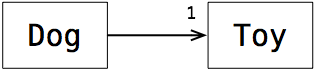
\includegraphics[width=1.5in]{singleassoc}
            \end{center}
        \item An \textbf{aggregation relationship} represents situations when the field type is a part of or belong to the class, and are represented with a diamond on the tail of the arrow. 
            \begin{center}
                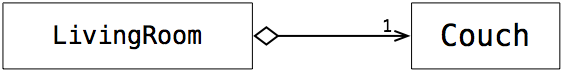
\includegraphics[width=2in]{singleagg}
            \end{center}
        \item If it is impossible to draw a dual arrowhead (such as when arrow tails are diamonds), the arrowheads are left off. 
        \item The \textbf{depends upon} association, represented by a simple dashed arrow, represents when a class uses constants or has local variables of a given type but does not have that type as a field. 
        \item In summary of the arrow types,
            \begin{center}
                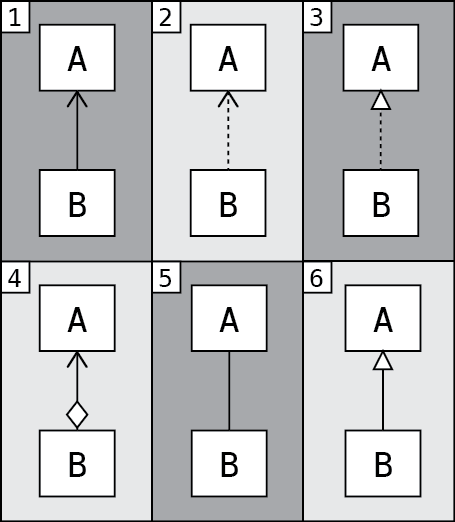
\includegraphics[width=2in]{arrowtypes}
            \end{center}
                \begin{enumerate}
                    \item $B$ is associated with $A$. 
                    \item $B$ depends on $A$. 
                    \item $B$ implements $A$.
                    \item $B$ is an aggregation of $A$. 
                    \item $B$ and $A$ have a bidirectional association.
                    \item $B$ extends $A$.
                \end{enumerate}
    \end{itemize}

    \subsection{Extracting Sequence Diagrams}
    \begin{itemize}
        \item A \textbf{sequence diagram} represents method excecution. 
        \item Each active object has a vertical \textbf{lifeline} labelled with the object name and type (superscript) with time increasing lower on the line. 
        \item Calls to methods are represented by horizontal lines labelled with the method name with paramaters. A box on a lifeline represents a method on the call stack, in this way arrows create and end boxes. There is an implicit lifeline leftwards of the leftmost arrow representing time, and calls from or returns to the rest of the program. 
        \item Calls to the same object (\textbf{self calls}) should create another box to the right of the object's box with a little round arrows going to and from it. 
        \item Loops are represented by large rectangles enclosing loop behavior. The loop
            \begin{lstlisting}
            for (X x : listofx) {method(x);}
            \end{lstlisting}
            will be represented by a large rectangle labelled \textit{loop listofx} in the top left corner, followed by the implicit \textit{getNext} call to listofx which returns $x$, and then the sequence diagram for \textit{method} using a lifeline for $x$. 
        \item Similarly, the diagram for 
            \begin{lstlisting}
            if (statement) {method();}
            \end{lstlisting}
            would be a rectangle labeled \textit{if (statement)} and enclosing the sequence diagram for \textit{method()}. 
        \item Other methods for loops use labels like \textit{loop [until listofx.hasNext() is false]} which is more similar to \textit{while}-type loops. Abbreviations are often used in these diagrams as well, the purpose of these diagrams is clarity first and foremost. 
    \end{itemize}
    
    \subsection{Implementing a Hierarchy, Simple Fields and Optional Sequences}
    \begin{itemize}
        \item When we implement associations as fields we may need to determine how exactly the associations are represented. For fields with cardinality $>1$, we must decide to implement them individually (only possible if the cardinality is fixed) or as a collection. 
        \item When implementing collections, the \textbf{Java Collections Framework} provides several options depeding on the collection's use case:
             \begin{itemize}
                 \item \textbf{List Interface} \\
                     Positional and allowing duplicates
                     \begin{itemize}
                         \item \textbf{ArrayList}:
                             Items stored in an array
                             \begin{itemize}
                                 \item Fast: append/get(1)
                                 \item Slow: insert/remove/contains/add or remove using iterator (n)
                             \end{itemize}
                         \item \textbf{LinkedList}:
                             Items not stored in an array
                             \begin{itemize}
                                 \item Fast: append/add or remove using iterator (1)
                                 \item Slow: insert/get/remove/contains (n)
                             \end{itemize}
                     \end{itemize}
                 \item \textbf{Set Interface} \\
                     Non-positional and disallowing duplicates
                     \begin{itemize}
                         \item \textbf{HashSet}:
                             Items are not ordered (iterator returns items in no order)
                             \begin{itemize}
                                 \item Fast: add/remove/contains (1)
                             \end{itemize}
                         \item \textbf{TreeSet}:
                             Items are ordered (iterator returns items in order)
                             \begin{itemize}
                                 \item Slow(-er than HashSet): add/remove/contains (log(n))
                             \end{itemize}
                     \end{itemize}
            \end{itemize}
    \end{itemize}

    \subsection{Overriding Equals and Hashcode}
    \begin{itemize}
        \item A \textbf{map} is a structure of key-value pairs. Pairs are inserted using the \textbf{put} method, values with the \textbf{get(key)} method, and a collection of keys with the \textbf{keyset} among others.
        \item A concrete subtype of map is the \textbf{HashMap}.
        \item HashMap's methods, among other Java operations determine equality with the \textbf{.equals} method which by default is the same as the \textbf{==} method. The == method compares if two objects are literally the same thing, which is not what we want to compare in general. Thus we must \textbf{override the equals method} in our objects to specify how exactly we would like our objects compared. 
        \item When we override the equals method, we must also override the HashCode method. 
    \end{itemize}

    \subsection{Implementing Bi-Directional Relationships and Sequence Diagrams}
    \begin{itemize}
        \item Consider a bi-directional association of arbitrary cardinality between $A$ and $B$. Every implementation of this has a similar form:
            \begin{enumerate}
                \item $A$ must have a collection of $B$ as a field, and $B$ must have a collection of $A$ as a field.
                \item In the class $A$, the relationship looks like
                    \begin{lstlisting}
                        class A {
                            Collection<B> listOfB;
                            public addB(B b){
                                if (!listOfB.contains(b)) {
                                    listOfB.add(b);
                                    b.addA(this);
                                }
                            }
                        }
                    \end{lstlisting}
                    and vice-versa in $B$. The order is important to avoid infinite recursion. 
            \end{enumerate}
        \item A bi-directional association of fixed cardinality would be similar, replacing list addition with setting the field value and the guard with field equality testing. Again, changing the order will give a recursion. 
        \item Implementing sequence diagrams is also fairly straightforward, the method is essentially encoded in the arrow labels and control flow rectangles. 
    \end{itemize}

    \newpage
    \section{Design}
    \subsection{Cohesion and Coupling}
 
    \begin{framed}
        \begin{center}
            Design Principle: The Single Responsibility Principle
        \end{center}
        Each abstraction (class or method) should have a single purpose or represent a single concept. A class contain the minimal amount of information to complete this purpose effectively. 
    \end{framed}

    \begin{itemize}
        \item If an abstraction has several purposes, it is lacking in \textbf{cohesion}. To improve the cohesion of the class, it's methods should be seperated into several classes of a single purpose and with only the data needed for those purposes. 
        \item \textbf{Coupling} refers to how indimately two abstractions are related. Coupling is acceptable if it only makes reference to the public interface of a module. Poor coupling is associations between implementations, or creating an excessive public interface as an afterthought of the implementation and is not essential to the purpose of the class. 
        \item Code duplication is another example of poor coupling. 
        \item In general, errors in well coupled code will be detected by tests and the compiler while errors in poorly coupled code will not. 
        \item One way to improve coupling is by applying concepts from functional programming. References to object attributes can sometimes be passed as functional paramaters, which can serve to remove unwarranted associations. Other ways to improve coupling could involve abstracting similar behaviors into a type hierarchy with a class representing the similarity in function between two modules. 
    \end{itemize}

    \subsection{Liskov Substitution Principle}
    \begin{framed}
        \begin{center}
            Design Principle: The Liskov Substitution Principle (LSP)
        \end{center}
        A sub-abstraction can be substituted for it's super-abstraction if it does not break the expectations set by it's super-abstractions. Unsubstitutible behaviors include
        \begin{itemize}
            \item Narrowing of domain (strengthening of preconditions)
            \item Widening of range (broadening of postconditions)
        \end{itemize}
    \end{framed}

    \begin{itemize}
        \item In Java the LSP can be violated if the REQUIRES clause of the subclass methods do not include some elements of the superclass, or if the EFFECTS clause of the subclass describes broader behavior than the superclass. 
        \item We can fix violations of the LSP by abstracting the essential behavior as an interface or abstract class, or alternatively by changing an \textit{extends} relationship to weaker \textit{uses} association. Either one of these allows us to relieve some expectations placed on a particular class and satsify the LSP. 
        \item Some tests which can help to determine if a substitution violates the LSP:
            \begin{itemize}
                \item \textbf{Substitution test:} Can the subtype be substituted as the supertype in Java's type systemm?
                \item \textbf{Concatentation test:} Does the subtype make sense as a noun preceding the supertype as an adjective?
                \item \textbf{IS-A test:} Is the subtype a special version of the supertype? This intuition based test is the most comprehensive. 
            \end{itemize}
            If the tests fail, it may be more prudent to represent this as a \textit{knows about} or \textit{has} type of association. 
    \end{itemize}

    \subsection{Refactoring}
    \begin{itemize}
        \item \textbf{Refactoring} is the process of making structural changes (not behavioral changes) to make our code more principled. 
        \item Refactoring is best done starting with exhaustive, passing tests. With a sufficient set of tests, we have complete domain to alter anything in our implementation without changing anything about the public interface. 
        \item It is also to refactor methods for readability, as more code is written the purpose of old code will be less obvious and potentially even less relevant. 
        \item It is important in larger scale projects, especially those with multiple contributors, that the public interface of abstractions be maintained and stable. Under our design principles, it is more important for sustainability to have well defined public interfaces at the outset than well designed private implementations because the former becomes hard or infeasible to change. 
    \end{itemize}

    \subsection{Composite Pattern/Singleton Pattern}
    \begin{framed}
        \begin{center}
            Design Principle: Design Patterns
        \end{center}
        Design patterns are broadly applicible and highly principled solutions to common problems in computer programming. Learning design patterns is a straightforward way to making principled solutions easier or effortless to write. 
    \end{framed}
    \begin{itemize}
        \item The \textbf{Composite Pattern} is an object oriented solution to hierarchy. 
        \item Elements of a hierarchy are represented as \textbf{composites} (nodes with children), \textbf{leaves} (nodes without children), and both are subtypes of a \textbf{component} which encodes the behavior of existing in the hierarchy. 
        \begin{center}
            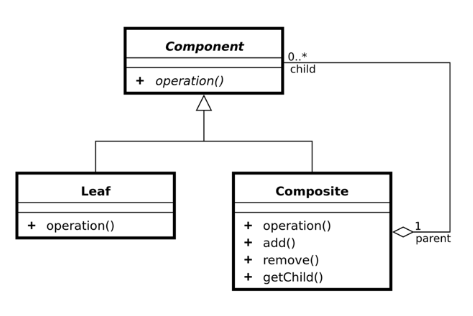
\includegraphics[width=3in]{composite} 
        \end{center}
        \item To write a composite pattern:
            \begin{enumerate}
                \item Determine the composite (the object which contains other objects)
                \item Detmine the leaves (the object that does not contain other objects)
                \item Write them to extend component, a abstract class or interface with a temlate for the operation(s)
                \item Equip the composite with a list of components and methods thereof
                \item Implement the operation(s) recursively over the list of components
            \end{enumerate}
        \item A related design pattern is the \textbf{singleton}, which ensures a class has only one instanceand to provide it with a global reference. 
            \begin{center}
                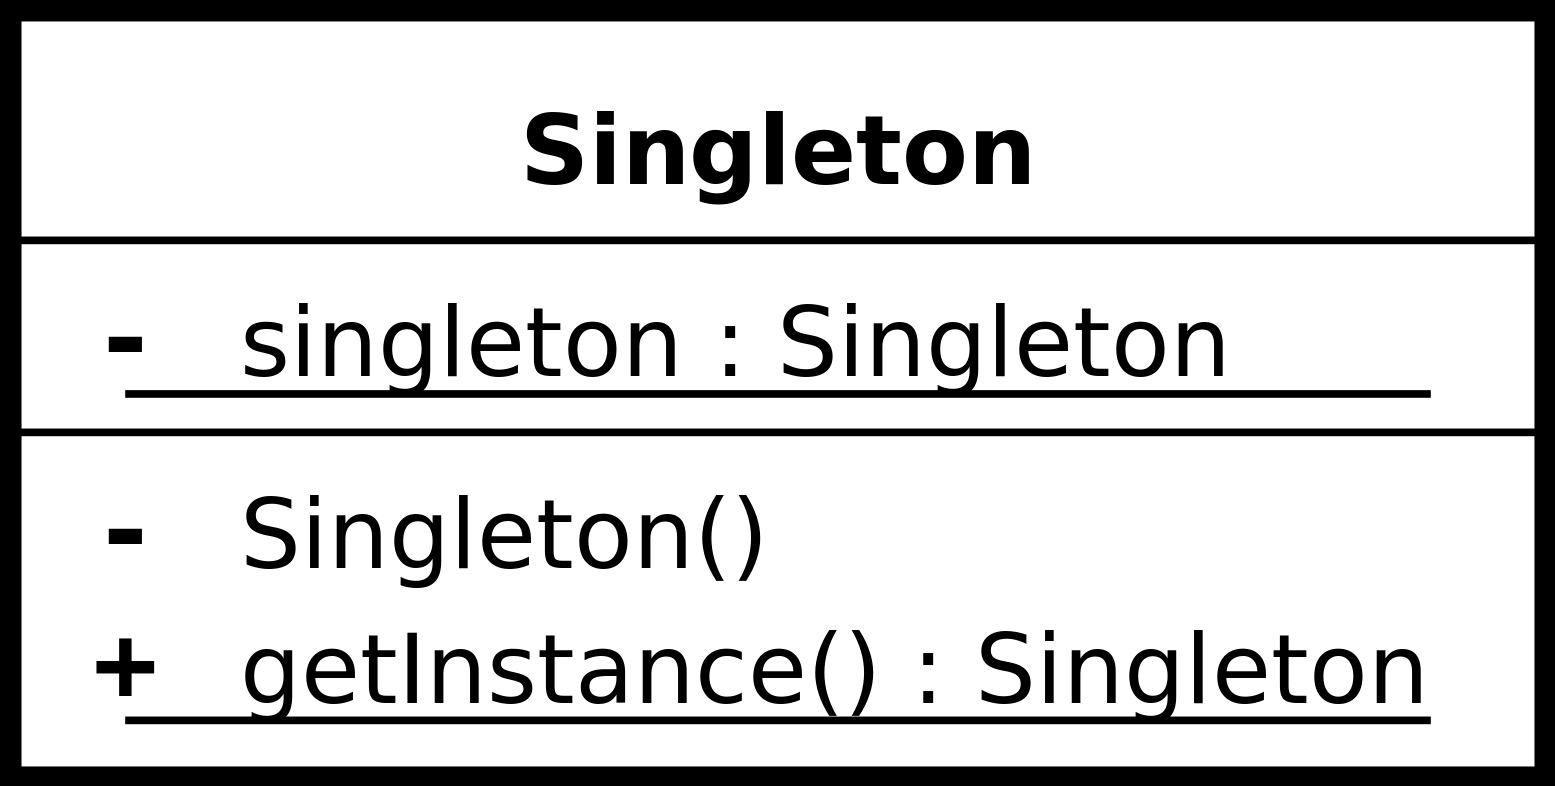
\includegraphics[width=1.4in]{singleton}
            \end{center}
        \item A singleton is achieved by equiping a class with a static, final reference to a singleton, a private constuctor and a static method accessing this reference. The only way to create a singleton is by the accessing method, and the accessing method gives a reference to exactly one singleton. One could also program behavior on the singleton creation (creation used pretty loosely here) or allow a finite number of singletons by removing the finality of the singleton and having more complicated behavior in the access method. The key to the singleton pattern is the private constructor so object creation is controlled. 
    \end{itemize}

    \subsection{Observer Pattern}
    \begin{itemize}
        \item The \textbf{Observer Pattern} is an object oriented solution for one object watching another. 
            \begin{center}
                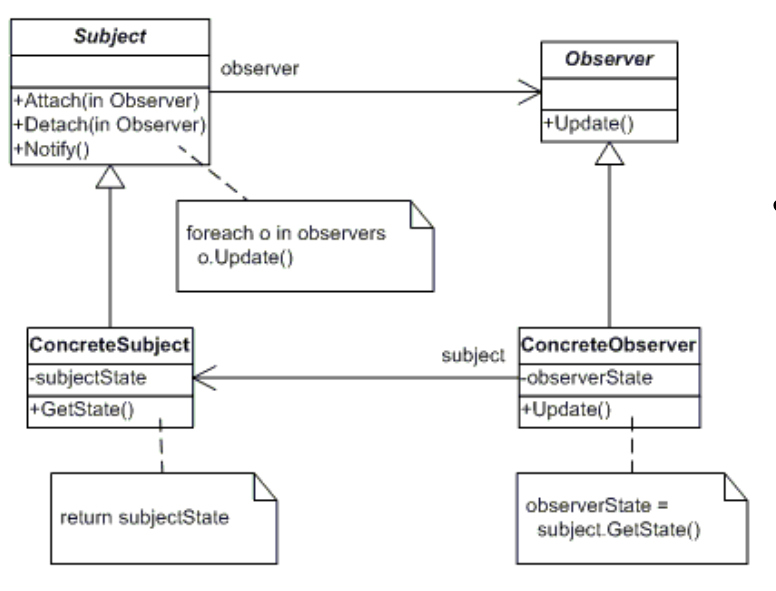
\includegraphics[width=3.4in]{observer}
            \end{center}
        \item The observer pattern takes place as follows:
            \begin{itemize}
                \item ConcreteSubjects are set up to know about Observers (an \textit{addObserver} method)
                \item When the ConcreteSubject does somehting of note it makes a call to \textit{notifyObservers}, which instructs all known observers to make a call to an abstract \textit{update} method accordingly. 
            \end{itemize}
        \item In this model the subject has the responsibility to \textbf{push} the information to the observers. Alternatively, another model would push a notification to observers that a change has occured and that the observers should \textbf{pull} information from some public \textit{getSubjectState} method instead. 
    \end{itemize}

    \subsection{Java's Observer}
    \begin{itemize}
        \item Java implements an Observer by default. The Subject is replaced by an \textbf{Observable} class and the Observer is replaced by an \textbf{Observer} interface. Barring these changes, it has the same notation as the figure in subsection 4.5. 
    \end{itemize}

    \subsection{Basic Iterator}
    \begin{itemize}
        \item The \textbf{Iterator Pattern} is an object oriented solution to iterating over a collection of sub-objects. 
        \item In Java, \textbf{Iterator$\langle E \rangle$} is an interface (with notable functions \textit{hasNext()} and \textit{E next()}) which represents something which can iterate over all of it's sub-objects of type $E$. 
        \item In Java Collections, Colleciton implements Iterable which represents something which can has an Iterator. There are Iterator subtypes for all of the subtypes of Collection such as a ArrayListIterator or a TreeSetIterator, which are ensured to be there by implementing tht Iterable interface. 
        \item Similarly if we would like to implement Iterable in a class $A$ over a sub-object $B$ (that is, have $A$ implement Iterable$\langle B \rangle$ we must implement the \textit{iterator()} method. In a simple case were we are already using a collection $c$, we can just return a premade iterator associated with that collection:
                \begin{lstlisting}
                    @Override
                    public Iterator<B> iterator() {
                        return c.iterator();
                    }
                \end{lstlisting}
            \item Iterable classes can use the for/each loop syntax. 
    \end{itemize}

    \subsection{Advanced Iterator}
    \begin{itemize}
        \item If the class is not using a collection, to implement iterable you must create your own custom iterator. 
        \item An instance of iterator is best implemented as an inner class (a class within another class which can see private data). This instance of iterator needs at a minimum to implement \textit{hasNext()} and \textit{next()}.
        \item One common situation for creating a custom iterator is when two collections need to be iterated over. It is possible to combine two default iterators in a custom iterator inner class.
    \end{itemize}

\end{document}










